\documentclass[a4paper]{article}
\usepackage{a4wide}
\usepackage{amsmath}
  \DeclareMathOperator*{\argmax}{arg\,max}
\usepackage{booktabs}
\usepackage{csquotes}
\usepackage{upquote}
\usepackage{float}
\usepackage{graphicx}
\usepackage{enumerate}
\usepackage{subcaption}
\usepackage{xcolor}
\usepackage{mcode}
\usepackage[numbered,framed]{matlab-prettifier}

\title{Pattern and Speech Recognition WS2015-16 \\ Exercise 2}
\author{Atanas Poibrenski(2554135), Marimuthu Kalimuthu(2557695), Furkat Kochkarov(2557017)}

\begin{document}

\maketitle

\section*{1 Preparation}
\subsection*{1.1 Loading and Plotting in the waveform}
\begin{enumerate}
	\item[\textbf{Ex.2}] Complete waveform.
	\begin{figure}[H]
		\begin{center}
			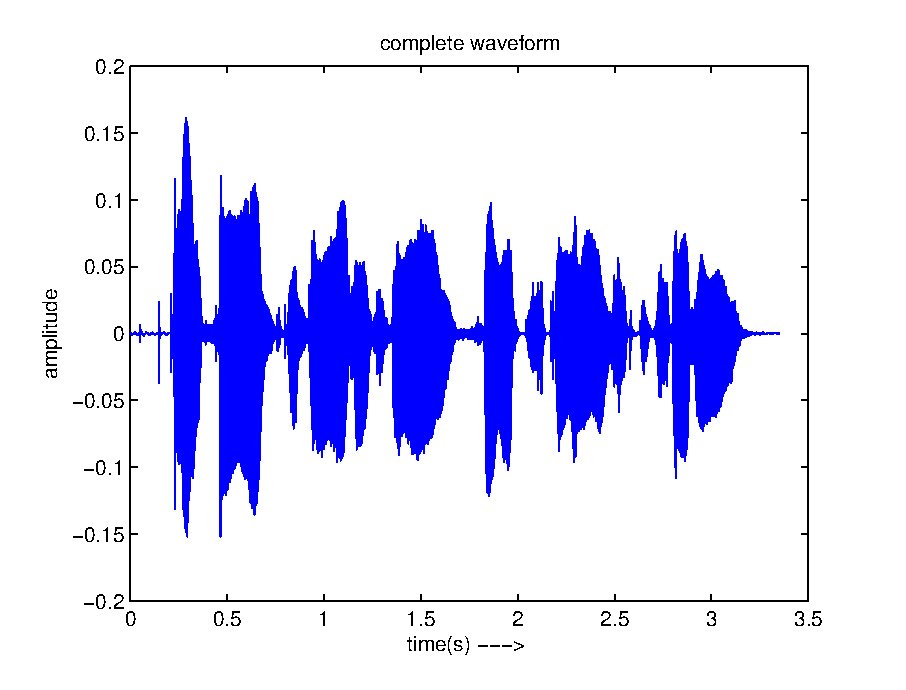
\includegraphics[width=0.85\textwidth]{ex2.eps}
			\caption{Complete waveform}\label{fig:comwavform}		
		\end{center}
	\end{figure}
	
	\item[\textbf{Ex.3}] Yes the same pattern is repeated multiple times in the signal. It roughly resembles the sawtooth waveform.
	\begin{figure}[H]
		\begin{center}
			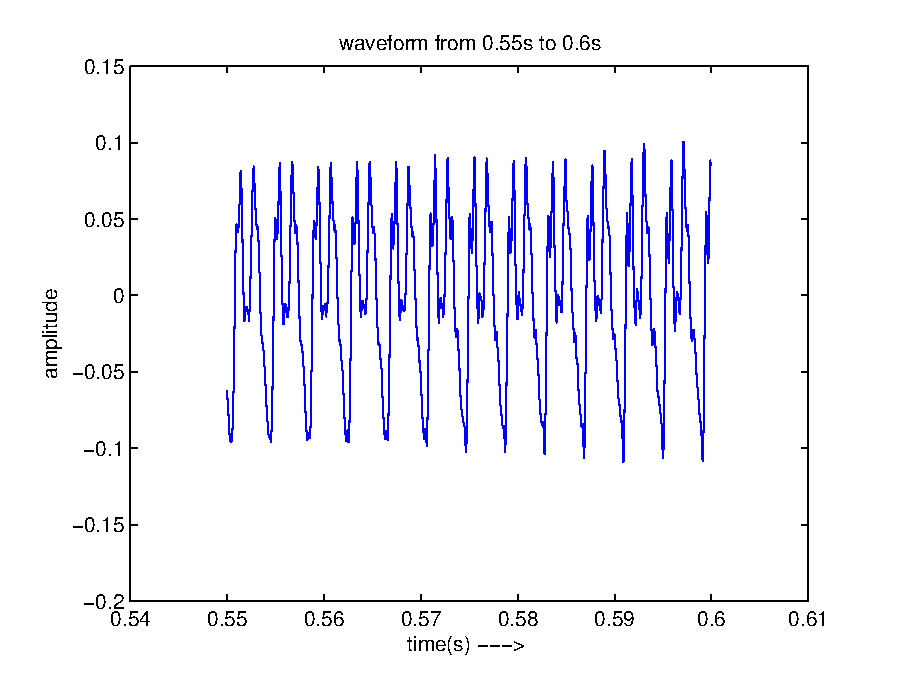
\includegraphics[width=0.85\textwidth]{ex3.eps}
			\caption{Waveform from 0.55s-0.6s}\label{fig:wav55}		
		\end{center}
	\end{figure}

\item[\textbf{Ex.4}] No pattern can be found in the signal.
\begin{figure}[H]
	\begin{center}
		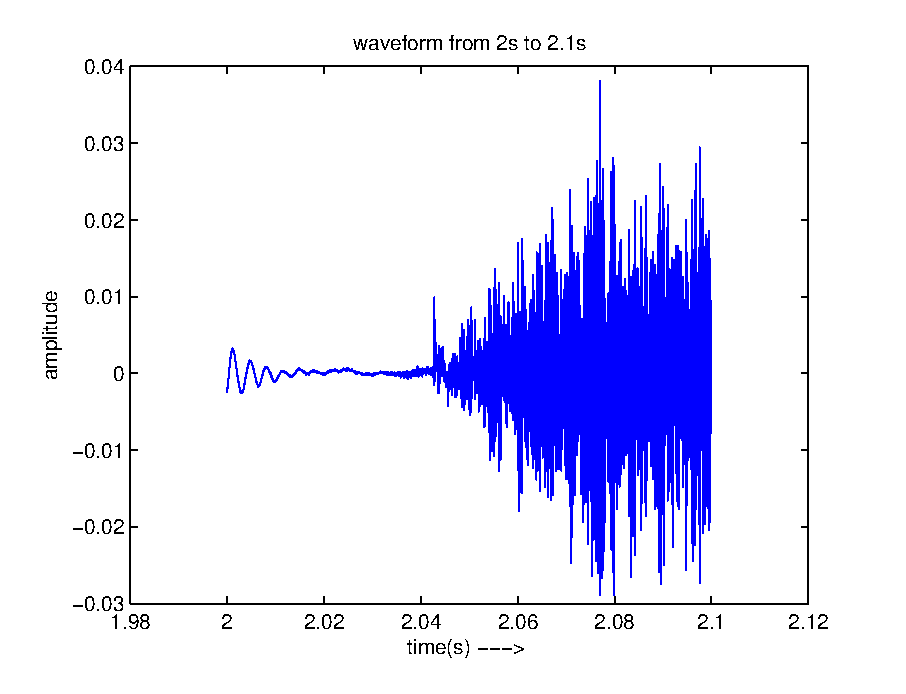
\includegraphics[width=0.8\textwidth]{ex4.eps}
		\caption{Waveform from 2s-2.1s}\label{fig:wav2}		
	\end{center}
\end{figure}
\end{enumerate}

\section*{2 Spectrum Analysis}
\subsection*{2.1 A reference plot}
\begin{enumerate}
\item[\textbf{Ex.5}] A spectrogram shows how the frequency content of a signal changes over time. It's a 2-dimensional function of amplitude (brightness or color) vs frequency (vertical axis) vs time (horizontal axis)

\begin{figure}[H]
	\begin{center}
		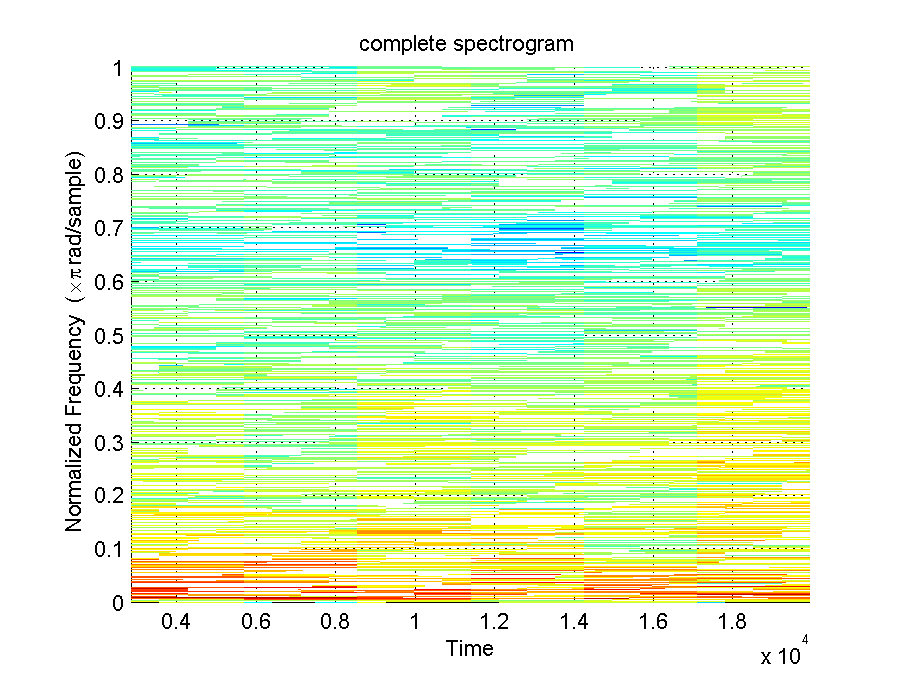
\includegraphics[width=0.85\textwidth]{ex5.eps}
		\caption{Spectrogram of the sample}\label{fig:spectro}		
	\end{center}
\end{figure}


\item[\textbf{Ex.6}] It is a voiced segment. \newline
\textit{Reason}: When producing voiced speech, the air exhaling out of lungs through trachea will be interrupted periodically by the vibrating vocal folds. Because of this, the glottal wave is generated that excites the speech production system resulting in voiced speech. Thus, when we observe at a speech signal waveform, if it looks \textit{nearly periodic in nature}, then it can be marked as voiced speech.

\begin{figure}[H]
	\begin{center}
		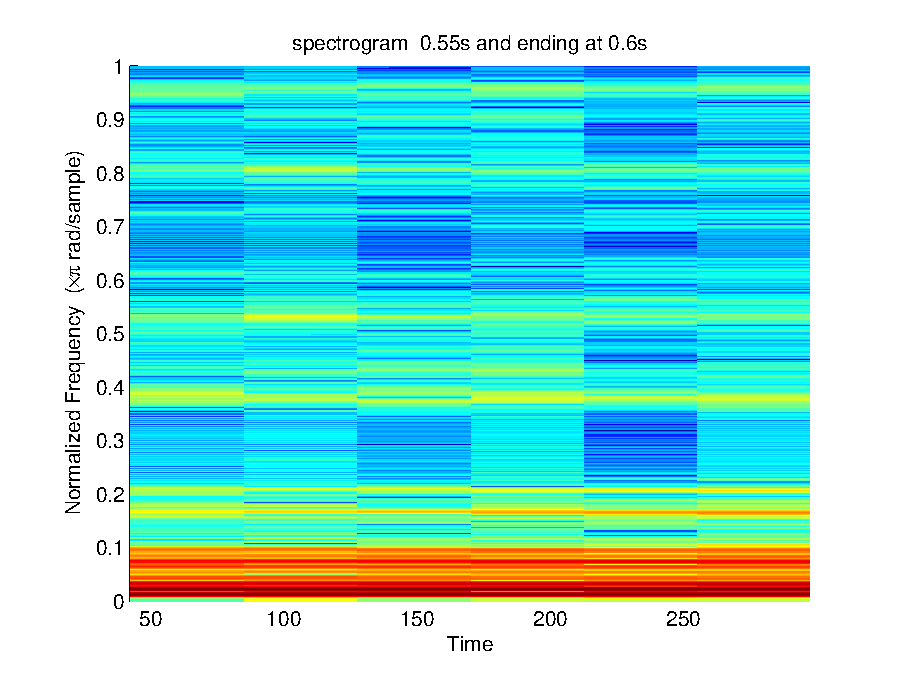
\includegraphics[width=0.65\textwidth]{ex6.eps}
		\caption{Spectrogram of the segment from 0.55s-0.6s}\label{fig:spectro55}		
	\end{center}
\end{figure}

\item[\textbf{Ex.7}] It is an unvoiced segment. \newline
\textit{Reason}: The waveform that we observe has no periodic pattern and is caused by some random noise. \\
During unvoiced speech duration, somewhere along the length of vocal tract, total or partial closure occurs resulting in obstruction of air flow completely or narrowly. This modification of airflow causes the vocal tract system to produce unvoiced speech.

\begin{figure}[H]
	\begin{center}
		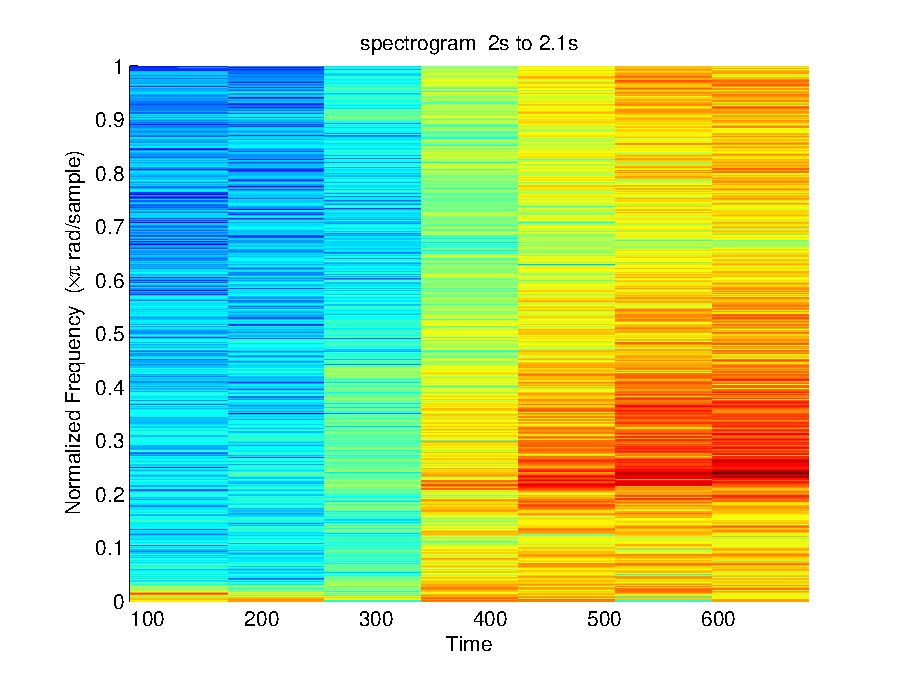
\includegraphics[width=0.6\textwidth]{ex7.eps}
		\caption{Spectrogram of the segment from 2s-2.1s}\label{fig:spectro2}		
	\end{center}
\end{figure}

\end{enumerate}


\subsection*{2.2 Compute spectrum}
\subsubsection*{2.2.1 windowing}

\begin{itemize}
	\item[\textbf{Ex.8}]
	\item Rectangular window : See ``rectWindow.m"
	\begin{figure}[H]
		\begin{center}
			\includegraphics[width=0.7\textwidth]{ex8_1.eps}
			\caption{Rectangular window}\label{fig:rectw}		
		\end{center}
	\end{figure}
	
	\item Hamming window : See ``hammingWindow.m"
		\begin{figure}[H]
			\begin{center}
				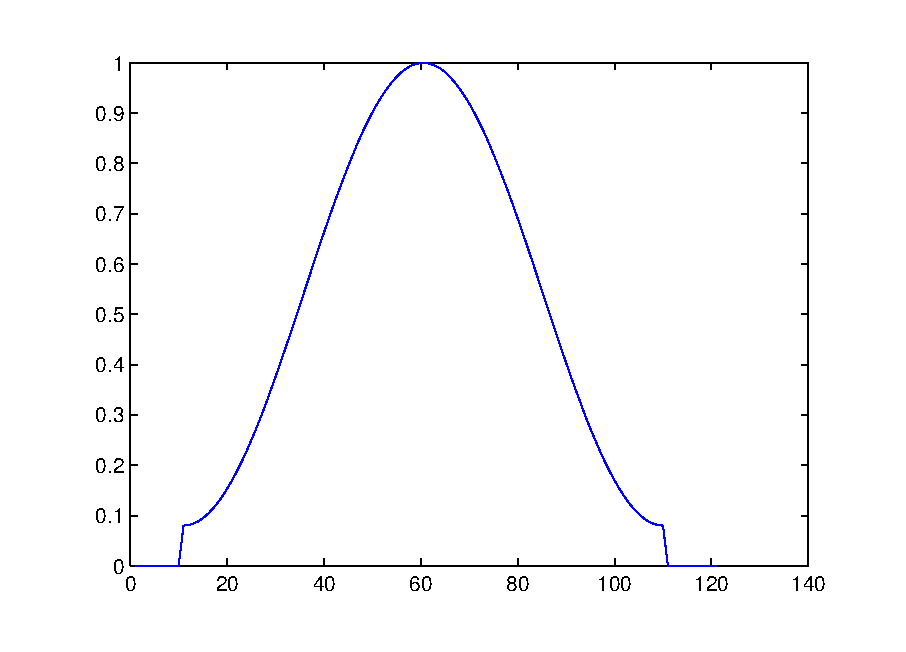
\includegraphics[width=0.7\textwidth]{ex8_2.eps}
				\caption{Hamming window}\label{fig:hammw}		
			\end{center}
		\end{figure}
		
\end{itemize}

\begin{enumerate}
\item[\textbf{Ex.9}]
It implies that we have an overlap of windows equivalent to the duration of frameshift. Here we will have an overlap of 5ms. We choose the hamming window because it produces much less spectral leakage.

\item[\textbf{Ex.10}] See ``applyHamming.m''

\end{enumerate}

\subsubsection*{2.2.2 Generate a spectrum section}
\begin{enumerate}
	\item[\textbf{Ex.11}]
	
	\begin{align*}
	ss &= \frac{frame\hspace{3pt}start\hspace{3pt}time}{frameshift} * \Bigg\{	\frac{frameshift}{length\hspace{3pt}of\hspace{3pt}x (ms)} \Bigg\} * (Number\hspace{3pt} of\hspace{3pt} samples\hspace{3pt} in\hspace{3pt} x) \\
	&= \frac{550}{5} * \frac{5}{3350} * 160800 \\
	&= 26400 \\
    \newline
	ee &= ss + \Bigg\{ \frac{winsize}{length\hspace{3pt}of\hspace{3pt}x (ms)} * (Number\hspace{3pt} of\hspace{3pt} samples\hspace{3pt} in\hspace{3pt} x) \Bigg\} \\
	&= 26400 + \bigg\{ \frac{25}{3350} * 160800 \bigg\} \\
	&= 27600
	\end{align*}
	
	So we have to use the index from 26400 to 27600.

	\item[\textbf{Ex.12}] Yes this result is expected because the signal is periodic and it is symmetric with respect to the center point of the x-axis. This represents the Nyquist frequency.
	
	\begin{figure}[H]
		\begin{center}
			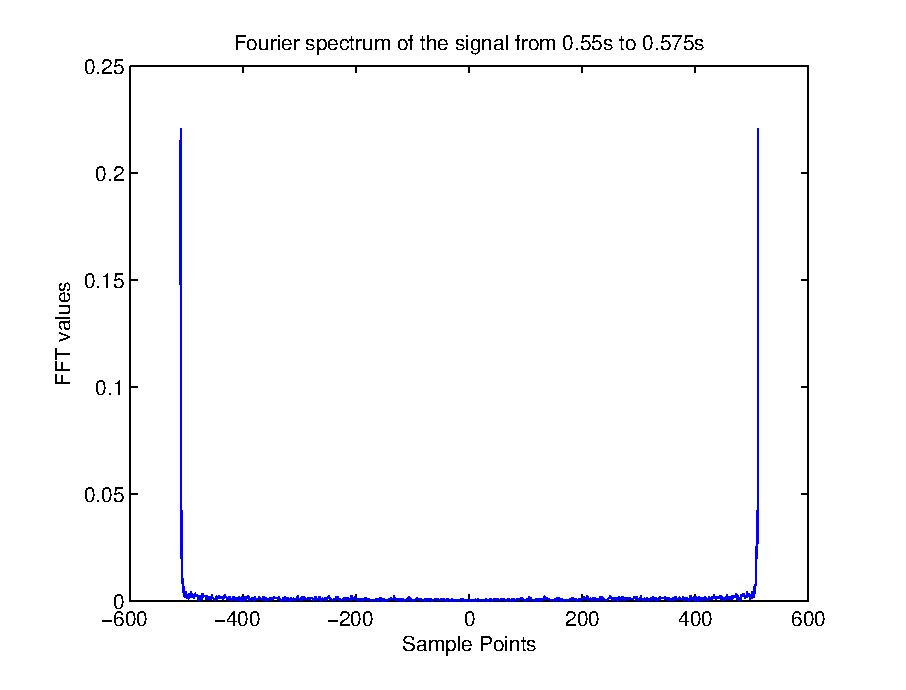
\includegraphics[width=0.85\textwidth]{ex12.eps}
			\caption{Fourier spectrum applied}\label{fig:fourier}		
		\end{center}
	\end{figure}

	
	\item[\textbf{Ex.13}] It helps to visualize the fourier transform with the zero-frequency component in the middle of the spectrum.
	\begin{figure}[H]
	\begin{center}
		\includegraphics[width=0.85\textwidth]{ex13.eps}
		\caption{FFT shifted}\label{fig:fftshift}		
	\end{center}
	\end{figure}
	\item[\textbf{Ex.14}] Since the signal is symmetric(periodic) in the fourier domain, we can just remove one part of the symmetry and keep the other part. See Figure \ref{fig:fourier}.
	
	\item[\textbf{Ex.15}] The \textit{x-axis} should represent the frequency. In order to achieve this, we should normalize the indices and multiply them by the sampling rate.  See Figure \ref{fig:fftshift}. Also see ``ex02.m"(line:89)
\end{enumerate}

\subsubsection*{2.2.3 Generate the power spectrum}
\begin{enumerate}
	\item[\textbf{Ex.16}] See ``powerSpectrum.m"
	\item[\textbf{Ex.17}] Power spectrum
	\begin{figure}[H]
		\begin{center}
			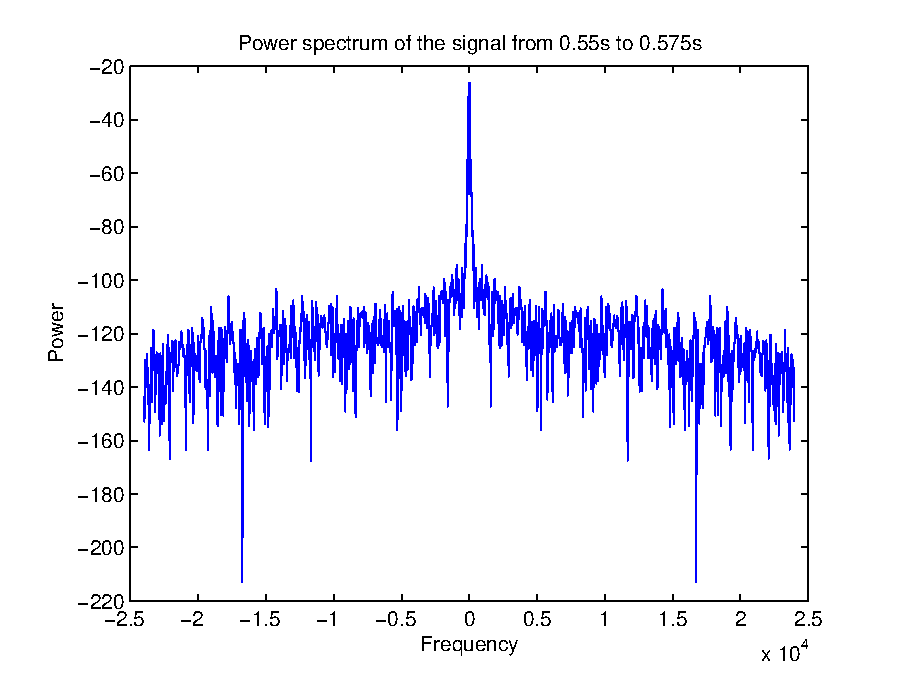
\includegraphics[width=0.85\textwidth]{ex17.eps}
			\caption{Power spectrum}\label{fig:powersp}		
		\end{center}
	\end{figure}
	
	\item[\textbf{Ex.18}]
	To plot a spectrogram we need \textit{time interval} together with the frequencies and the corresponding amplitudes.
	The power spectrum can provide time interval, frequencies, and power per frequency. \newline
	Since power is proportional to the square of amplitude, we can compute the corresponding amplitudes for each frequency.
\end{enumerate}

\section*{Bonus - From spectrum to mel-cepstrum}

\begin{enumerate}
	\item[\textbf{Ex.19}] Applying discrete cosine transform.
	\begin{figure}[H]
		\begin{center}
			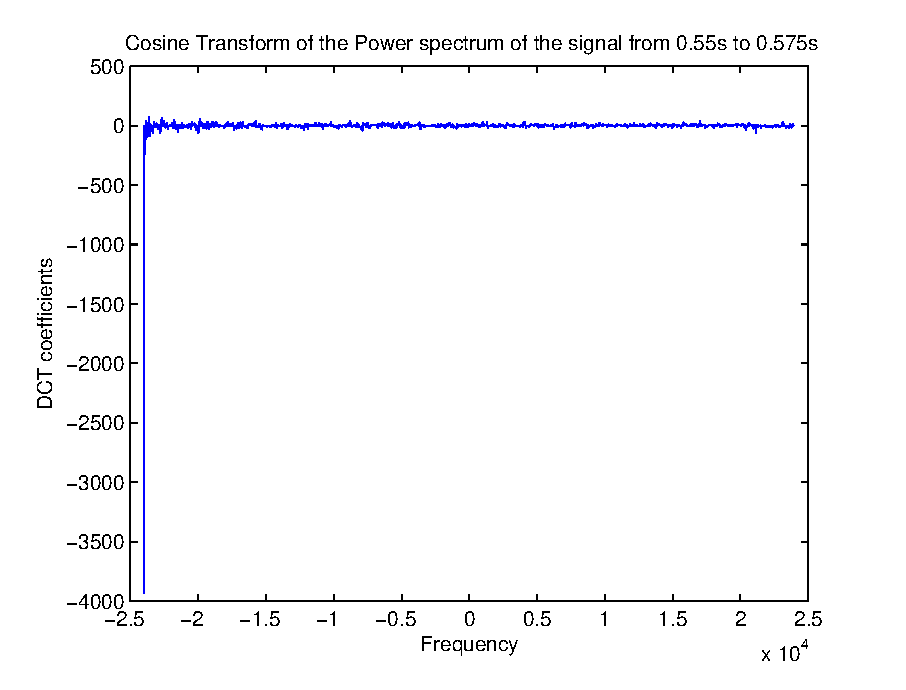
\includegraphics[width=0.52\textwidth]{ex19.eps}
			\caption{DCT to 0.55s}\label{fig:dct}	
		\end{center}
	\end{figure}
\end{enumerate}

%to include whole matlab file in the report
%\lstinputlisting{../code/ex02.m}
%\vspace{1em}


%to include a sample matlab code
%\begin{lstlisting}
% 	%return area of a triangle%
%	function [Area] = Area(a,b,c)
%	s = (a+b+c)/2;
%	Area = sqrt(s(s-a)*(s-b)*(s-c));
%	\end{lstlisting}



\end{document}
